\documentclass[12pt]{article} % For LaTeX2e
\usepackage{latex_template,times}
\usepackage{hyperref}
\usepackage{url}
\usepackage{bigints}
\usepackage{natbib}
\usepackage{amsmath}
\usepackage{amssymb}
\usepackage{euler}
\usepackage[]{hyperref}
\usepackage{prettyref}
\usepackage{mathtools}
\usepackage{csvsimple}
\usepackage{booktabs}
\usepackage{microtype}
\usepackage{doi}
\usepackage{bm}
\usepackage{listings}
\lstset{escapeinside={(*@}{@*)}}
\usepackage{inconsolata}
\usepackage[author={Chen}]{pdfcomment}
\newcommand{\chenc}[1]{\pdfcomment[author=Chen,color={1 0.5 0.5},subject={#1}]{#1}}
\newcommand{\hayden}[1]{\pdfcomment[author=Dania,color={1 1 1},subject={#1}]{#1}}
\newcommand{\tina}[1]{\pdfcomment[author=Joyce,color={1 0 1},subject={#1}]{#1}}
\DeclarePairedDelimiter{\norm}{\lVert}{\rVert}
% in dvi it only seems to use urlcolor !!!!
\hypersetup{colorlinks,linkcolor=blue,citecolor=blue,pagecolor=blue,%
            urlcolor=magenta,filecolor=magenta,breaklinks,%
            dvips,bookmarks,bookmarksopen}
%\documentstyle[nips14submit_09,times,art10]{article} % For LaTeX 2.09

%\author{Chen C che5002 480458339, Yutong Cao ycao5602 470347494,***}
\title{Assignment 2}

\newcommand{\fix}{\marginpar{FIX}}
\newcommand{\new}{\marginpar{NEW}}
\newcommand{\svm}{\textsc{svm}}
\newcommand{\loss}{\ell}
\newcommand{\rhoo}{\rho_{+1}}
\newcommand{\rhoz}{\rho_{-1}}
\newcommand{\mnist}{fashion-\textsc{mnist}}
\usepackage{amsthm}
\nipsfinalcopy % Uncomment for camera-ready version
\lstdefinestyle{python-idle-code}{%
  language=Python,                   % the language
  showspaces=false,
  showtabs=false,
  breaklines=true,
  showstringspaces=false,
  breakatwhitespace=true,
  basicstyle=\normalsize\ttfamily,   % size of the fonts for the code
  % Color settings to match IDLE style
  keywordstyle=\color{orange},       % core keywords
  keywordstyle={[2]\color{purple2}}, % built-ins
  stringstyle=\color{green2},
  commentstyle=\color{red},
  upquote=true,                      % requires textcomp
}
%\lstloadlanguages{Python}
\lstset{
  style={python-idle-code},
  showstringspaces=false,  % true by default for python
  % tabsize=4,
}
\lstset{
float=table,
stringstyle=\color{orange},
basicstyle=\color{black}\footnotesize\ttfamily,
numbers=left,
numberstyle=\tiny\color{brown},
%numberstyle=\small,
numbersep=8pt,
%frame = leftline,
breaklines=true,
firstnumber=1,
language=python,
numberstyle=\tiny\color{brown},
keywordstyle=\color{blue},
commentstyle=\color{green!50!black}}
\renewcommand{\lstlistingname}{Algorithm}
\begin{document}

\author{%
 \begin{tabular}{rl}
  Tutors:& Nicholas James, Zhuozhuo Tu, Liu Liu\\ \\
Group members: & Yutong Cao (ycao5602) 470347494,\\
& Chen Chen (cche5002) 480458339,\\
& Yixiong Fang (yfan5798) 480133344.
\end{tabular}
}

\maketitle



\begin{abstract}
{\color{red}Please improve the English here.}

This report documents three algorithms against class-dependent classification noise (\textsc{ccn}) based on the soft-margin support vector machines. We first preprocess the datsets by normalisation and principal component analysis, and estimate the flip rates by a density ratio method. We then propose a new kernel that is designed against \textsc{ccn} base on Expectation Maximisation . We gave a rigorous proof that the proposed kernel is positive definite. In addition, we implement the Importance Reweighting method proposed by \citet{liu2016classification}. Our third algorithm is to heuristically relabel the contaminated labels by a pre-training model. Our numerical experiment applies regression to estimate the complexity of the three algorithms. We also use nonparametric hypothesis test to compares their accuracies. We find the first two algorithms provides similar accuracy. However, the Expectation Maximisation has a shorter running time. The heuristically proposed relabelling method gives inconsistent result during resampling.
\end{abstract}
\tableofcontents
\section{Introduction}
This report documents our modifications to the soft-margin support vector machine~(\svm) to improve its performance against class-dependent classification noise (\textsc{ccn}).

The capability of learning with label noise is crucial for training machine learning models. According to the Law of Large Numbers \citep{hardle2007applied}, the empirical risk converges to the expected risk asymptotically as the sample size approaches infinity. However, classification labels in large datset can be easily corrupted. For example, images  are sometimes labelled manually by employing casual staff with minimal training. In this case, training a classification models using these images requires special treatment that accounts for noisy labels. Section~\ref{method} proposes three such treatments based on \svm\ to increase the accuracy with presence of \textsc{ccn}.

%maybe move to related work
%Usually there is a trade-off between the data complexity and the data quality ({\color{red} reference!}). Weakly supervised learning methods are introduced to handle this kind of problems ({\color{red} reference!}). For example, positive and unlabelled learning and semi-supervised learning are designed to trade data complexity for data quality. They both make use of a small set of correct data to train a model. Also there is learning with noisy labels, on the contrary, trades data quality for data complexity. It learns a model with a large amount of noisy data. In this assignment, we only focused on the latter.

 %For both datsets, the flip rates are given.
Section~\ref{1st} proposed a learning method by deriving a new loss function using Expectation Maximisation \citep[p.423]{Bishop:2006:PRM:1162264}. This method models the label noise using a Bernoulli distribution, and includes the label noise information into the loss function of \svm. This method is first studied by \citet{pmlr-v20-biggio11} for random classification noise (\textsc{rcn}), and we extended it to \textsc{ccn}.

Section~\ref{3rd} implements importance reweighting proposed by \citet{liu2016classification}. This method uses a reweighting coefficient to reweight the loss function for each sample point. We fit \svm s with the given noisy data. We then implement cross-validation of \svm\ models to predict the probabilities of classifying each sample, and then use these probabilities to calculate the weightings.

Section~\ref{2nd} introduces a filtering approach based on the work of \citet{brodley1996identifying}. This method follows the heuristic observation that the predicted probability of a sample point with wrong label is usually close to 0.5, where our model is not able to classify confidently. In the meanwhile, the predicted classification result of contaminated label is likely to be different from the observed label.  We then exclude the potential contaminated data points and train the model again with the remaining data which seems to be cleaner.

To fairly compare these three approaches of attacking noisy data, all of the three methods implement the same base classification algorithm---\svm. We use \svm\ because it is proved to has a strong generalisation ability \citep{NIPS2012_4500,Seeger:2003:PGE:944919.944929,Cortes1995}, and usually gives high classification accuracy when turned properly \citep{Fernandez-Delgado:2014:WNH:2627435.2697065}. In addition, \svm\ is more susceptible to label noise than many other algorithms \citep{frenay2014classification}, so we can better assess our modification to the original classification algorithm.
%As a result,  it is not considered to be robust to label noise ({\color{red} gives reference})

Section~\ref{result} applies the three methods proposed in Section~\ref{method} to two sets of noisy data with binary labels, both containing $10,000$ images. The first datset is a subset of the \mnist\ database and the second datset is from the \textsc{cifer} database. For each datset, Section~\ref{result} also compares the simulation results, including accuracy and running times, from the three methods. In addition, we estimate the flip rate~$\rhoz$, $\rhoo$ using the method proposed by \citet{liu2016classification}.
%We did not use the estimated values in our classification experiments as the true rates are provided.
Section~\ref{result} also compares our estimation with the true values.
\section{Related work}
Many recent literature discusses the topic of learning with label noise. One popular approach is to use classification algorithms that are proved to be robust to label noise. \citet{frenay2014classification} reported their findings that $0-1$ loss and least-squares loss are robust loss functions to uniform label noise. %compared $179$ classifiers from $17$ families on $121$ datsets.
They also found the method of bagging is robust against label noise. Bagging detect the contaminated samples by estimating the variability of its base classifier when including and excluding them. %We chose not to use the robust loss functions as the corresponding classification models may not produce satisfying classification accuracy as \textsc{svm}.
%But we used a bagging-like technique by sampling multiple times and averaging the predicted probabilities to generate better and more stable predictions.
\citet{frenay2014classification} also discussed filtering methods for learning with label noise. These methods remove mislabelled data before training a final model. Our second model follows this idea by excluding data points with vague predictions. Instead of removing the contaminated candidates directly, \citet{yang2018adasampling} proposed a filter-like method that estimating the probability of mislabelling for each sample.

These approaches mentioned above do not require noise rates. Although this makes the approaches general, the methods may not be able to handle highly contaminated datset, especially when the noise rates are given. \citet{pmlr-v20-biggio11} applies Expectation Maximisation method to fit data with \textsc{rcn}. This method reformulates the loss function to include noise rate information. The label noise is not usually observed. They use the expected value as an estimation of unobserved labels contaminated by noise. Section~\ref{1st} extends his method to solve problems with \textsc{ccn}. The idea behind this method is straightforward and intuitive, but  simulation results in Section~\ref{result} finds it is less accurate than the method of importance reweighting proposed by \citet{liu2016classification}. \citet{liu2016classification} assigned a weight to each sample according to its probability of being contaminated. These probabilities are estimated from a pre-train model. They also provided an efficient method for estimating the noise rate. However, the need of fitting the model twice makes the method of reweighting slow.

\section{Methods}\label{method}


\subsection{Base model: support vector machine}\label{sec:over}
We use \textsc{svm} with Gaussian kernel as the base classification method for this task because of its generalisation ability.

Let vector~$x_i$ to represent the $i$th image in the dataset. The corresponding true classification labels~$y_i$ of images are corrupted by \textsc{ccn} and the we only observe the contaminated labels~$s_i$. The clean and observed label~$y_i$ and $s_i$ are both binary variables drawn from set~$\left\{-1,1\right\}$. We use $n$ to denote the number of samples, and $p$ to denote the number of feature of a input datset.

\textsc{svm} with Gaussian kernel was first published by \citet{Boser:1992:TAO:130385.130401}.
\citet{Cortes1995} proposed an improvement on the original \textsc{svm} with soft-margin  to  avoid over-fitting problem. The \textsc{svm} is to minimise the Hinge loss function
\begin{equation*}
\left[{\frac {1}{n}}\sum _{i=1}^{n}\max \left(0,1-y_{i}(w\cdot x_{i}-b)\right)\right]+\lambda \lVert w\rVert ^{2}.
\end{equation*}
Here, $w$ is the weighting factor, $b$ is a constant. We classify the $i$th image into category~$1$ or~$-1$ when $w\cdot x_{i}-b\geq1$ or $w\cdot x_{i}-b\leq-1$, respectively. This loss function not only penalises points that misclassified, but also points that are closed to the dividing hyperplane, with a regularisation term~$\lambda \lVert w\rVert ^{2}$. The decision function of \svm\ is
\begin{equation}\label{eq:decision}
 g(x_{i})=\text{sign}(w\cdot x_{i}-b).
\end{equation}

\subsubsection{Support vector machine resists over-fitting}\label{sec:over}
\citet{Fernandez-Delgado:2014:WNH:2627435.2697065} asserted that \svm\ was very likely to be one of the most powerful classifiers, by comparing 179 classification algorithms over 121 large datsets. The distances between data points and the dividing hyperplane give an intuitive estimate of the generalisation ability of the trained \svm\ model \citep{hastie01statisticallearning}.


we use \svm\ as our classification method as of its strong generalisation ability. %In this image classification assignment, we do not observe the true  labels~$y_i$. 
This section proposes three different approaches to modify ordinary \svm\ to attack label noise problem. However, we do not have access to a test datset with true labels~$(x_i,y_i)$ to verify the generalisation ability of our three different models, which are all trained by noisy data~$(x_i,s_i)$. In \svm , the gap between hyperplane and the training datset provides a natural and `free' metric of its generalisation ability  \citep{hastie01statisticallearning}, and hence use of test datset is not mandatory. Using this geometry factor as well as probably approximately correct learning framework,  \citet{NIPS2012_4500} proved that the  \svm\ models have strong generalisation ability. Further,  \citep{Cortes1995,Seeger:2003:PGE:944919.944929} also shows the strong generalisation ability from different perspectives.

\subsubsection{Support vector machine is not robust to label noise}

The other reason of implementing \svm\ as the base algorithm is that the hinge loss function makes \svm\ not robust against label noise \citep{frenay2014classification}. Nevertheless, our proposed modifications in Sections~\ref{1st}, \ref{3rd} and~\ref{2nd} give accurate classification results as shown in Section~\ref{result}. If we implement a robust algorithm, e.g. deep neural networks, then one could argue that the flip rates had minimal impact on the classification result anyway. Hence whether our methods perform well would become a mystery.

%As we are not focusing on the effect of robust classification methods on learning with label noise. Using hinge loss should remove this effect and let us focus on the label noise methods we use instead of the natural robust property of certain loss functions.

\subsection{Preprocess}\label{preproc}
\subsubsection{Photometric normalisation improves classification performance}
We applied Photometric normalisation suggested by \citet{jonsson2002support} to re-scaled the image datsets to have mean of zero and standard deviation of one. This scaling visually removes the brightness difference among different images, and dramatically improves the performance of Gaussian kernel \svm . This preprocess procedure is mandatory because Gaussian kernel is a radius based kernel, which only performs well when data are on a similar scale \citep{jonsson2002support}.

\subsubsection{Principle component analysis reduces dimensionality}
For the large \textsc{cifer} datset, we applied principle component analysis (\textsc{pca}) to decrease the dimensionality of the datset from $3072$ to $100$. Although the dimensionality is reduced by $97\%$, the remaining $3\%$ features explains more than $85\%$ of the variance in the datset.

No \textsc{pca} is applied to the \mnist\ datset because the dimensionality ($p=784$) is already low comparing with the number of training samples ($n=8,000$) in the datset. Nevertheless, for the purpose of estimating the flip rates~$\rhoz$ and~$\rhoo$ only (i.e. Section~\ref{method2} only), we applied \textsc{pca} to decrease the number of features of \mnist\ datset to $50$. The reason of applying \textsc{pca} is that the method estimating density ratio in Section~\ref{method2}is slow when the number of features is large, especially when grid search the optimal hyperparameters .

\subsection{The original datset is balanced} \label{sec:1}
Define random variables~$Y$ and $S$ as the true and contaminated binary classification label of a random image vector~$X$, respectively. The assignment instruction states the probabilities~$\rhoz=P(S=1|Y=-1)=0.2$ and $\rhoo=P(S=-1|Y=1)=0.4$.
%, where $S$ are the contaminated classification labels and $Y$ are the true classification labels.
The contaminated data has $40.0\%$ labels~$S$ as one (i.e. $P(S=1)$). Using this factor and the law of total probability
\begin{equation*}
P(S=1)=P(S=1|Y=1)P(Y=1)+P(S=1|Y=-1)P(Y=-1),
\end{equation*}
An observe label can either be $1$ or $-1$, $P(S=1|Y=1)=1-P(S=-1|Y=1)$,
\begin{equation*}
P(S=1)=\left[1-P(S=-1|Y=1)\right]P(Y=1)+P(S=1|Y=-1)P(Y=-1)
\end{equation*}
Knowing the flip rates~$P(S=-1|Y=1)=0.4$ and $P(S=1|Y=-1)=0.2$
\begin{equation}
P(S=1)=0.6P(Y=1)+0.2\left[1-P(Y=1)\right]=0.4, \label{eq:ps}
\end{equation}
which implies $P(Y=1)=P(Y=-1)=0.5$. Thus, the original classification problem is balanced.
In addition, define the Bernoulli random variable~$\epsilon(S)$ with the means 
\begin{equation}\label{eq:e1}
  E(\epsilon(S=1))=P(Y=-1|S=1)=0.5\times0.2/0.4=0.25.  
\end{equation}
and 
\begin{equation}\label{eq:em1}
  E(\epsilon(S=-1))=P(Y=1|S=-1)=0.5\times0.4/0.6=1/3.  
\end{equation}

This random variable~$\epsilon$ describe the unobserved random label noise. Hence the expectation
\begin{equation}
    E\epsilon(S)=P(Y=-1|S=1)P(S=1)+P(Y=1|S=-1)P(S=-1)
    %=0.25\times 0.4+1/3\times0.6
    =0.3.\label{eq:exp}
\end{equation}

\subsection{Flip rates estimation}\label{method2}
We apply techniques proposed by \citet{liu2016classification} to estimate the flip rates~$\rhoz$ and $\rhoo$. The technique consists of two steps---firstly, we estimate probability~$P_{D_\rho}(S|X)$; secondly, we estimate the flip rates~$\rhoz$ and $\rhoo$ using the probability~$P_{D_\rho}(S|X)$.
To use this technique, we need to assume that $\rho_{S}\leq P_{D_\rho}(-S|X)$ holds.


\subsubsection{Density ratio method estimates conditional probability}\label{method22}
Bayesian formula expands the conditional probability~$P_{D_\rho}(S=s|X)$ to
\begin{equation}
   P_{D_\rho}(S=s|X)=\frac{P_{D_\rho}(X|S=s)P_{D_\rho}(S=s)}{P_{D_\rho}(X)}.\label{eq:baye}
\end{equation}
Here the probability~$P_{D_\rho}(S=s)$ is given by equation~\eqref{eq:ps}. We use the density ratio method proposed by \citet{DBLP:journals/jmlr/KanamoriHS09} to estimate the ratio~${P_{D_\rho}(X|S=s)}/{P_{D_\rho}(X)}$.

Define a Gaussian Kernel
\begin{equation}\label{eq:gauss}
k(x_i,x_j)=\exp(-\gamma\norm{x_i-x_j}).
\end{equation}
Then the set~$\{k(X,x_j) \}_j$ forms the basis function for the probability space of ${P_{D_\rho}(X|S=s)}/{P_{D_\rho}(X)}$. Hence we can model the probability by a linear combination of the basis functions
\begin{equation*}
   \frac{P_{D_\rho}(X|S=s)}{P_{D_\rho}(X)}=\sum_j \alpha_{sj} k(X,x_j) \text{ where }\alpha_{sj}>0.%\label{eq:baye2}
\end{equation*}
To compute coefficients~$\alpha_{sj}$, we treat the centres~$x_j$ and the number of basis functions as hyperparameters and minimises the objective function
\begin{equation*}
  \min_\alpha \bigintss \left(\frac{P_{D_\rho}(X|S=s)}{P_{D_\rho}(X)}-\sum_j \alpha_{sj} k(X,x_j)\right)^2P_{D_\rho}(X)dx \text{ where }\alpha_{sj}>0.
\end{equation*}
Treating terms without coefficients~$\alpha_{sj}$ as constants and applying Monte Carlo to transform the integration into a summation, this objective function further simplifies to a constrained quadratic programming problem about coefficients~$\alpha_{sj}$. Solving this quadratic programming problem gives coefficients~$\alpha_{sj}$, and hence an approximation of the ratio~${P_{D_\rho}(X|S=s)}/{P_{D_\rho}(X)}$. Substituting this ratio into Bayesian formula~\eqref{eq:baye} gives required conditional probability~$P_{D_\rho}(S=s|X)$.

The advantage of the density ratio method is to avoid estimating probabilities~${P_{D_\rho}(X|S=s)}$ and~${P_{D_\rho}(X)}$. Estimating these are usually difficult for high dimensional data~$X$, due to curse of dimensionality.


\subsubsection{Minimum of conditional probability estimates flip rates}\label{method23}
Theorem~4 proposed by \citet{liu2016classification} estimates the flips rates using the global minimum of conditional probability~~$P_{D_\rho}(S=s|X)$ computed in Section~\ref{method22}
\begin{equation*}\label{eq:fliprate}
\rho_s=\min _X P_{D_\rho}(S=s|X).
\end{equation*}

As our sample size is large ($10,000$), the minimal probability of the samples approximates the global minimum well.

The method proposed here requires tuning a few hyperparameters by grid search. Thus, later sections do not use this density ratio method for the speed of our algorithms.
In addition, when numerically computing these flip rates, we only use the datset \mnist. This datset is less complex in features comparing with \textsc{cifar}, and hence allows us to grid search the best hyperparameter faster. To further avoid overfitting, we applied \textsc{pca} to decreases the number of features to $50$ when estimating flip rates.

As the true flips rates~$\rhoz$ and $\rhoo$ are given, here and after, we use the true flip rates~$\rhoz=0.2$ and $\rhoo=0.4$ in Sections~\ref{1st}, \ref{3rd} and~\ref{2nd}.


\subsection{Method 1: Expectation Maximisation}\label{1st}
This section extends the Expectation Maximisation algorithm proposed by \citet{pmlr-v20-biggio11} to improve ordinary \svm\ against labels noises, with mathematical justifications.
%---the given label noise where flip rates~$P(S=1|Y=-1)=0.2$ and~$P(S=-1|Y=1)=0.4$ seems to be marginally different to a random label noise with flip rate~$P(S=1|Y=-1)=P(S=-1|Y=1)=0.3$ for \textsc{svm}.
\subsubsection{Expectation Maximisation derives loss function}
The original algorithm proposed by \citet{pmlr-v20-biggio11} was proposed to study classification problems with label noise where the flip rate $\rhoz=\rhoo$ and we extend it to manage the case dependent label noise where the flip rates are different.

Recall the dual problem of an \textsc{svm} is to maximise
\begin{equation}
   f(c_{1}\ldots c_{n})=\sum _{i=1}^{n}c_{i}-{\frac {1}{2}}\sum _{i=1}^{n}\sum _{j=1}^{n}y_{i}c_{i}k(x_{i},x_{j})y_{j}c_{j}, \label{eq:dual}
\end{equation}
\begin{math}
{\text{subject to }}\sum _{i=1}^{n}c_{i}y_{i}=0,\,{\text{and }}0\leq c_{i}\leq {\frac {1}{2n\lambda }}\;{\text{for all }}i.
\end{math}
Here $y_i$ and $x_i$ are the labels and features of the $i$th image, $c_i$ is the $i$th Lagrangian multiplier, $\lambda$ is a regularisation parameter,and $k(x_i,x_j)$ is the Gaussian Kernel product~\eqref{eq:gauss} of vectors~$x_i$ and~$x_j$.

\subsubsection{Bernoulli random variable models th latent label noise}
The nature of \textsc{ccn} implies that the latent class-dependent noises~$\epsilon(s_i)$ follows Bernoulli distributions with the parameters given as mean~\eqref{eq:e1} and~\eqref{eq:em1}, depending on the value of label~$s_i$. The observed label~$s_i$ is correct if and only if the noise~$\epsilon(s_i)=0$. For the $i$th image, it is straightforward to verify that
\begin{equation*}
y_i=s_i(1-2\epsilon(s_i)).
\end{equation*}

Substituting this expression of label noise into loss function~\eqref{eq:dual} gives
\begin{equation}
   f(c_{1}\ldots c_{n})=\sum _{i=1}^{n}c_{i}-{\frac {1}{2}}\sum _{i=1}^{n}\sum _{j=1}^{n}S_{i}c_{i}k(x_{i},x_{j})S_{j}c_{j}(1-2\epsilon(s_i))(1-2\epsilon(s_j)). \label{eq:dual2}
\end{equation}
This loss function involves latent random variables. For a similar  but simpler problem with \textsc{rcn}, \citet{pmlr-v20-biggio11} applied the technique of Expectation Maximisation, which uses the expected value of the loss function as the objective function for optimisation algorithms.

Here, when $i=j$, the expectation~$E(1-2\epsilon(s_i))(1-2\epsilon(s_j))=1-4E\epsilon(s_j)+4E\epsilon(s_j^2)=1$.
When $i\neq j$, by substituting these expectations~\eqref{eq:exp} from Section~\ref{sec:1}, the expectation~$E(1-2\epsilon(s_i))(1-2\epsilon(s_j))=(1-2E\epsilon(s_i))(1-2E\epsilon(s_j))=0.16$.

Define the correction term~$m_{ij}:=E(1-2\epsilon(s_i))(1-2\epsilon(s_j))$. The diagonal entries~$m_{ii}=1$, and the off diagonal entries~$m_{ij}=0.16$ when indexes~$i\neq j$. Taking the expected values of the loss function~\eqref{eq:dual2}
\begin{equation}
   Ef(c_{1}\ldots c_{n})=\sum _{i=1}^{n}c_{i}-{\frac {1}{2}}\sum _{i=1}^{n}\sum _{j=1}^{n}S_{i}c_{i}k(x_{i},x_{j})S_{j}c_{j}m_{ij}. \label{eq:dual3}
\end{equation}

\subsubsection{Modifying kernel improves robustness against label noise} \label{sec:mod}

Comparing this loss function and the ordinary loss function of \svm\ \eqref{eq:dual}, the only difference is to replace the kernel products~$k(x_i,x_j)$ with our new proposed kernel~$k^*_{ij}:=k(x_i,x_j)m_{ij}$. Define matrix~$K$ as a matrix with $(i,j)$th entry being~$k(x_i,x_j)$. Similarly, Define matrix~$M$ as a matrix with $(i,j)$th entry being~$m_{ij}$. We implemented this modification by a Hadamard product~$K\circ M$ in \texttt{Python}:
\begin{lstlisting}[caption=Customised kernel for Expectation Maximisation Algorithm, label=matn1]
def my_kernel(X, Y):
    #parameter calculated from rhos  
    S=0.84
    #Only apply M when fitting the model but not evaluating decisions
    if np.array_equal(X,Y):
        N = X.shape[0]
        M=(1-S)*np.ones((N,N))+S*np.eye(N)
    else:
        M=1    
    pairwise_sq_dists = cdist(X, Y, 'sqeuclidean')
    K = exp(-gamma*pairwise_sq_dists)*M
    return K
#fit the model
clf = svm.SVC(kernel=my_kernel)
clf.fit(X_train,y_train)
\end{lstlisting}
When evaluating classification decisions for test data, we apply the ordinary Gaussian kernel~\eqref{eq:gauss} because we aim to predict labels with no noise. 
\subsubsection{Proof: proposed kernel matrix is positive definite} \label{sec:prove}
This section proves the kernel~$k^*_{ij}$ proposed in Section~\ref{sec:mod} is positive definite. This property is very important for many reasons. For example, if a kernel is not positive definite (or positive semidefinite), then it will not map to an inner product of the Hilbert space. Not having an inner product implies \svm\ cannot apply the kernel trick~\citep{Theodoridis:2008:PRF:1457541}, hence fitting the model becomes infeasible. To prove this kernel is positive definite, we only need to show the matrix~$K\circ M$ is positive definite.
\begin{proof}
Let $\vec x$ be any real vector in  $\mathbb{R}^n$. Line~$7$ of Algorithm~\ref{matn1} decompose matrix~$M=M_1+M_2$ where $M_1:=\texttt{(1-S)*np.ones((N,N))}$ and $M_2:=\texttt{S*np.eye(N)}$. The rank of  matrix~$M_1$ is one, hence matrix~$M_1$ only has one nontrivial eigenvalues. We further observe this nontrivial eigenvalue is $1-S>0$ corresponding to eigenvector~$\vec 1$. Hence matrix~$M_1$ is positive semidefinite
\begin{equation}\label{eq:p0}
    X^TM_1X\geq 0.
\end{equation}
Also, the matrix $M_2$ has exactly one repeated eigenvalue of $S>0$ with multiplicity~$n$, so it is positive definite
\begin{equation}\label{eq:p1}
    X^TM_2X>0.
\end{equation}
Substituting inequality~\eqref{eq:p0} and~\eqref{eq:p1} into the inner product
\begin{equation*}
    X^TMX=X^T(M_1+M_2)X=X^TM_1X+X^TM_2X>0.
\end{equation*}
Thus, the correction matrix~$M$ is positive definite.

Gaussian kernel~\eqref{eq:gauss} is a positive definite kernel. Consequently, its kernel matrix~$K$ is a positive definite matrix.

The matrix corresponding to our proposed kernel is $K\circ M$. As matrices~$K$ and $M$ are both positive definite, Schur product theorem \citep{Schur1911} implies that their Hadamard product~$K\circ M$ is also positive definite. So the proposed kernel~$k^*_{ij}$ is positive definite, and hence useful for \svm  s \citep{Theodoridis:2008:PRF:1457541}.
\end{proof}

%\subsubsection{Additional regularisation}


%This soft-margin \textsc{svm} is sub-optimal for our problem. We have a large set of data ($10,000$) comparing with the number of features ($784$). Hence, we build a modified \textsc{svm} that aims to minimise the following Hinge loss
%\begin{equation}
%\left[{\frac {1}{n}}\sum _{i=1}^{n}\max \left(0,10-y_{i}(w\cdot x_{i}-b)\right)\right]+\lambda \lVert %w\rVert ^{2}.   \label{eq:pri}
%\end{equation}
%The modified constant~$10$ requires the predictor~$w\cdot x_{i}-b$ to be as extreme as possible, i.e., it penalises wrongly classified samples. Moreover, it even penalises correctly classified samples with small gaps between data points and the dividing hyper-plane being small.
%Define $\zeta _{i}:=\max \left(0,10-y_{i}(w\cdot x_{i}-b)\right)$. The prime problem of Hinge loss~\eqref{eq:pri} becomes a minimisation of
%\begin{equation}
%{\frac {1}{n}}\sum _{i=1}^{n}\zeta _{i}+\lambda \|w\|^{2}
%{\text{ subject to }}y_{i}(w\cdot x_{i}-b)\geq 10-\zeta _{i}\,{\text{ and }}\,\zeta _{i}\geq 0,\,{\text{for all }}i. \label{eq:pri2}
%\end{equation}
%The modification is inspired by observing that the regularisation parameter~$\lambda$ has a negligible impact on the classification results for this problem. Hence we have more than enough data to train this complex model without over fitting.

%The modified \textsc{svm} aims to make the algorithm more robust to label noise, even though it may enlarge the generalisation error. Nevertheless, the large datset will assure us the generalisation error is within a reasonable magnitude.
%The parameters~$c_i$ are Lagrangian multipliers that enforcing the condition~$y_{i}(w\cdot x_{i}-b)\geq 10-\zeta _{i}$ in prime problem~\eqref{eq:pri2}.

%With this modification, the dual problem~\eqref{eq:dual3} of the loss function~\eqref{eq:pri} becomes
%\begin{equation*}
%   Ef(c_{1}\ldots c_{n})=10\sum _{i=1}^{n}c_{i}-{\frac {1}{2}}\sum _{i=1}^{n}\sum %_{j=1}^{n}S_{i}c_{i}k(x_{i},x_{j})S_{j}c_{j}m_{ij}. \label{eq:dual3}
%\end{equation*}
%From the dual prospective, we are weakening the contributions of the contaminated labels~$s_i$, hence making the algorithm more robust.



%This method gives us an accuracy of $94.6\%$ on the testing data.


\subsection{Method 2: Importance Reweighting} \label{3rd}
This section applies theorems proved by \citet{liu2016classification} to construct a weighted loss that includes noise information~$\rhoz$ and $\rhoo$.

\subsubsection{Sigmoid function estimates conditional probability}\label{sigmoid}
Define $D$ to be the probability density function of the clean data~$(X,Y)$ and $D_\rho$ to be that of contaminated data~$(X,S)$.

This section estimates the conditional probability~$P_{D_\rho}(S=y|X)$.

\citet{liu2016classification} provided three methods to estimate the conditional probability~$P_{D_\rho}(S=y|X)$.
The first method implements a probabilistic regresion model.
The second and third method both implement Bayesian formula~\eqref{eq:baye}.
\begin{equation*}
   P_{D_\rho}(S=y|X)=\frac{P_{D_\rho}(x|S=y)P_{D_\rho}(S=y)}{P(X)}.
\end{equation*}
However, the two methods are computationally different. The formal method requires to estimate two density functions~$P_{D_\rho}(X|S=y)$ and~$P(X)$ by kernel smoothing. Our datsets are high dimensional ($784$ and $3072$), so kernel smoothing suffers from the curse of dimensionality. The later method avoids kernel smoothing by estimating the ratio~$P_{D_\rho}(x|S=y)/P(X)$ directly through density ratio method \citep{liu2016classification}. For example, Section~\ref{method2} applies this method to estimate the flip rates~$\rhoz$ and $\rhoo$. Despite of the need of additional hyperparameters,  \citet{Sugiyama10densityratio} claims that the density ratio method is ``equivalent to the regression problem''. To keep our model simple and more interpretable, we implement a probabilistic regression model proposed in by \citet[Section~5.1]{liu2016classification}.

We apply probability estimation method proposed by \citet{Platt99probabilisticoutputs}. We first fit a pre-training model using an ordinary \svm . We then estimate the parameters of an additional logistic regression model to map the pre-training \svm\ outputs into probabilities. We apply this approach rather than traditional logistic regression because Remark 1 given by \citet{liu2016classification} indicates the logistic regression ``does not perform well''.

\subsubsection{Reweighting coefficient improves robustness against label noise}
To improve the robustness against label noise, \citet{liu2016classification} construct a reweighting coefficient vector~
\begin{equation}
\beta(X,Y,S)=\frac{P_D(Y|X)}{P_{D_\rho}(S|X)}. \label{beta}
\end{equation}
%in  to represent the expected risk if we can find the value of $\beta$
%where $D$ is the distribution of  and $D_\rho$ is the distribution of .
%\begin{eqnarray*}
%R_{l,D}(f) &=& \mathbb{E}_{(X,Y)\sim D}[l(f(X),Y)]\\
%           &=& \sum_{y}\int{P_D(X,Y=y)l(f(X),Y=y)}dX \\
%           &=& \sum_{y}\int{P_{D_\rho}(X,S=y)\frac{P_D(X,Y=y)}{P_{D_\rho}(X,S=y)}l(f(X),Y=y)}dX\\
%           &=& \mathbb{E}_{(X,S)\sim D_\rho}[\frac{P_D(X,Y=y)}{P_{D_\rho}(X,S=y)}l(f(X),S)]\\
%           &=& \mathbb{E}_{(X,S)\sim D_\rho}
%              [\beta l(f(X),S)] \\
%           &=& R_{\beta l,D_\rho}(f)
%\end{eqnarray*}
%Where $\beta=\frac{P_D(X,Y)}{P_{D_\rho}(X,S)}=\frac{P_D(Y|X)}{P_{D_\rho}(S|X)}$ as the distribution of $X$ does not change between $D_\rho$ and $D$.
%Now we can .
%Although we can make an approximation for $D_\rho$ using the given data, we can not approximate the distribution $D$ directly.
%We need to represent $P_D(Y|X)$ using $P_{D_\rho}(S|X)$ and the noise rates.
%\begin{equation}
%    \begin{aligned}
%    P(S=y|X) &= P(Y=y,S=y|X)+P(Y=-y,S=y|X)\\
%               &= P(S=y|X,Y=y)P(Y=y|X)
%                  +P(S=y|X,Y=-y)P(Y=-y|X)\\
%               &= (1-\rho_{y})P(Y=y|X)+\rho_{-y}[1-P(Y=y|X)]\\
%               &= (1-\rho_{y}-\rho{-y})P(Y=y|X)+\rho_{-y}
%    \end{aligned}
%\end{equation}
$\beta(X,Y,S)$ is set to be $0$ when $P_{D_\rho}(S|X)=0$.
With the assumption $\rhoo+\rhoz<1$ on flip rates, \citet{liu2016classification} also derive the distribution of the unobserved  true label using the observed label~$S$, the flip rates~$\rho_{0}$ and $\rho_{1}$
\begin{equation}
    P_D(Y=y|X)=\frac{P_{D_\rho}(S=y|X)-\rho_{-y}}{1-\rho_{y}-\rho_{-y}}.
\end{equation}
Substitute this estimation into the weighting coefficient~\eqref{beta}:
\begin{equation} \label{eq:weighting}
    \beta(X,Y,S)=\frac{P_{D_\rho}(S=y|X)-\rho_{-y}}{(1-\rho_{y}-\rho_{-y})P_{D_\rho}(S=y|X)}.
\end{equation}
Further substituting the conditional probability~$P_{D_\rho}(S=y|X)$ estimated in Section~\ref{sigmoid} gives reweighting coefficient~$\beta(X,Y,S)$.
Recall from equation~\eqref{eq:decision} that  $g$ is the decision function.
Reweighting coefficient~$\beta(X,Y,S)$ is then used to estimate the expected risk~$R_{\loss,D}(g)$ in the with the empirical risk $R_{\loss,D_\rho}(g)$
\begin{equation}
R_{\loss,D}(g) = R_{\beta \loss,D_\rho}(g). \label{eq:loss}
\end{equation}
This loss function allows us to estimate the true loss function~$R_{\loss,D}(g)$ without knowing the true labels~$Y$.

\subsection{Method 3: heuristic approach by relabelling}\label{2nd}
Method 3 implements a pre-training \textsc{svm} to select a subset of samples that are `cleaner'.
%\subsubsection{Hinge loss is robust against label noise}

\subsubsection{Conditional probability filters samples}\label{2nd2}
Ordinary \textsc{svm} only gives a classification without revealing a probability that indicates the confidence of classification.
\citet{Wu03probabilityestimates} proposed a five-fold cross-validation method to calculate the classification probabilities~$P(Y=1|X)$ for \textsc{svm}.
Using this method, we calculated the probability~$P(Y=1|X)$ with label noise by a pre-training \textsc{svm} with Gaussian kernel. Recall from equation~\eqref{eq:decision} that we use $g(X)$ to denote the decision made by this \svm .

Each datset has $10,000$ samples.
For each datset, we find the $1/3$ and $2/3$ percentiles of the sample conditional probability~$P(Y=1|X)$, denoted as as $P(Y=1|X_{(1/3)})$ and $P(Y=1|X_{(2/3)})$, respectively.
We only use a subset of samples where the predicted probability is very high or very low
\begin{equation}\label{eq:filter}
\left\{X|P(Y=1|X)\geq P(Y=1|X_{(1/3)}) \cup P(Y=1|X)\leq P(Y=1|X_{(2/3)}) \right\}.
\end{equation}
This method is inspired by the fact that the contaminated samples are more likely to have a probability~$P(Y=1|X)$ close to $0.5$. One third of sample are truncated because of the error rate~$P(\epsilon=1)=0.3\approx 1/3$. Note that this subset of sample is imbalanced.

\subsubsection{Pre-training model corrects labels}
We fit our model using the predictions~$g(X)$ rather than contaminated labels~$S$, because the way we filtered samples  assure us exactly half of predictions~$g(X)$ in the filtered samples~\eqref{eq:filter}  are ones.
Using a balanced data is important because section~\ref{sec:1} shows that the original datset is also balanced. In addition, filtered samples~\eqref{eq:filter} have  predicted probabilities far from $0.5$. Hence, the pre-training \svm\ are confident with its predictions~$g(X)$.
Training our \textsc{svm} with Gaussian Kernel again with this balanced subset of relabeled data gives the result.

Define the indicator function~$I_{g(X)=S} \in \left\{0,1\right\}$ as the binary scalar indicating whether decision made~$g(X)$ is the same as the observed labels~$S$. With this definition, the expression~$2I_{g(X)=S}-1$ is $-1$ when $g(X)\neq S$ and is $1$ when $g(X)=S$.  The model proposed in this section is equivalent to minimise the loss function~\eqref{eq:loss} with the weighting coefficient
\begin{equation*}
\beta\begin{cases}
2I_{g(X)=S}-1 & \text{when }P({Y}|X)\leq P(Y=1|X_{(1/3)}) \cup P({Y}|X)\geq P(Y=1|X_{(2/3)}),\\
0 & \text{when }P(Y=1|X_{(1/3)})<P({Y}|X)<P(Y=1|X_{(2/3)}).
\end{cases}
\end{equation*}
This approach is purely empirical. Thus, the prediction made by this model is neither guaranteed to be unbiased nor with bounded variance asymptotically.

This method gives us an accuracy of $95.0\%$ on the testing data.
%\subsubsection{Hinge loss if robust against label noise}


\subsection{Tuning hyperparameters}
The hyperparameters are tuned using coordinate descent \citep{hastie01statisticallearning}. Recall from equation~\eqref{eq:exp} that the total noise rate is 0.3. Hence,  the objective is to achieve an accuracy of $70\%$ when training the contaminated datsets~$(X,S)$. Intuitively, this is a necessary but not sufficient condition of tuning a `perfect' model---if the selected model with tuned hyperparameters perfect fits the clean data $(X,Y)$, then this model would predict the contaminated label~$S$ with a accuracy~$70\%$.

We choose the initial Kernel parameter for Gaussian Kernel~$\gamma$  to maximise the variance of the all kernel products~$k(x_i,x_j)$ over all $i,j$. 
This initial value assures us parameter~$\gamma$ is within the correct order: if parameter~$\gamma$ is very small, then the kernel~\eqref{eq:gauss} will approach one; if parameter~$\gamma$ is very large, then the kernel~\eqref{eq:gauss} will approach zero. In both situations, the variance of all kernel products~$k(x_i,x_j)$ is small.

The initial value of regularisation parameter~$\lambda$ is chosen as $1$.
The gradient is estimated by finite difference method.
The model seems to be insensitive to the regularisation parameter~$\lambda$.

Our model tends to be resist to over-fitting for three reasons. Most importantly, as discussed in Section~\ref{sec:over}, soft-margin \svm\ is known to have a strong generalisation ability \citep{NIPS2012_4500,Cortes1995,Seeger:2003:PGE:944919.944929}. Also, we select the hyperparameter of our model so that it predicts the contaminated label~$S$ with a accuracy~$70\%$, not $100\%$. Thirdly, the number of features~$p$ ($784$ for \mnist\ and $100$ for \textsc{pca} proprocessed \textsc{cifar}) is small comparing with the sample size ($8,000$).

\subsection{Bootstrap constructs confidence intervals and hypothesis tests}
Let $A_{ij}$ be the accuracy generated from our {$i$}th algorithm from the $j$th Monte-Carlo simulation. This section provides us a tool to compare the accuracy~$A_{ij}$ for the three proposed algorithms.
\subsubsection{Bootstrapping percentile confidence intervals}\label{ci}
To systematically compare the accuracy of the three methods introduced in Sections~\ref{1st}, \ref{3rd} and~\ref{2nd}, we construct the $95\%$ bootstrapping percentile confidence intervals for a set of $16$ accuracy results~$A$. The idea of bootstrapping  is straightforward---we resample a subset of $8$ samples among the sample space of the $16$ accuracy results and calculate their mean. We repeat this process $1000$ times. The $2.5\%$ and $97.5\%$ percentiles of the $1000$ re-sampled means are then the bootstrapping percentile confidence interval
\begin{equation}
({A}^*_{2.5}, {A}^*_{97.5}), \label{eq:boot}
\end{equation}
where $A^*_{\alpha}$ is the $\alpha$ percentile of the bootstrapped distribution from our sample space with $16$ accuracy result from Monte-Carlo simulations.

Bootstrapping does not require the sample space follows specific distributions. We apply this nonparametric method to construct confidence interval here because we do not know about the exact distributions of accuracy~$A$.

\subsubsection{Kolmogorov-Smirnov test compares the accuracy of algorithms}\label{sec:ks}
We implement the Kolmogorov-Smirnov test to test the hypothesis that the algorithms proposed in Section~\ref{method} have different accuracy.  Again, Kolmogorov-Smirnov test is distribution free, so we do not need to know the distributions of the evaluation metrics.

We define the empirical distribution of accuracy results generated by algorithm~$i$ as
\begin{equation}\label{epdf}
  \hat{F}_{i}(x)=\frac{1}{n}\sum_{j=1}^{16}I_{A_{ij} \leq x}.
\end{equation}
The test statistic is the supremum among the differences of the empirical distribution generated using empirical distribution~\eqref{epdf} of $i_1$th and $i_2$th algorithm \citep{Walck:1996cca}
\begin{equation}\label{teststatistic}
D=\sup _{x}\left|F_{i_1}(x)-F_{i_2}(x)\right|.
\end{equation}
We compare the test statistics~$D$ with the critical value of $0.433$, which corresponds to $16$ samples and a $95\%$ of confidence level. We reject the null hypotheses that the two algorithms produce the same accuracy~$A$ with $95\%$ confidence level if the test statistics~$D>0.433$.
%The technique is also applied to perform one tail test to test whether $i_1$th algorithm is more accurate than $i_2$th algorithm. In this case, the test statistic is the supremum
%\begin{equation}\label{teststatistic}
%D^+=\sup _{x}F_{i_1}(x)-F_{i_2}(x).
%\end{equation}
\section{Experiments}\label{result}
{\color{red} TODO compare photos
discuss pca
write captions.
please write good sentences.
perhaps imitate what the lecturer wrote in his paper}
\subsection{Experiment Setting}
To provide a more rigorous evaluation on performance, we train the model $16$ times for each method on each dataset. We then calculate the mean, standard deviation $95\%$ and confidence intervals of the $16$ results.
We randomly select $80\%$ of the training samples in each simulation.
To reduce the running time, we use multi-threading programming and train the $16$ models simultaneously. 

As machine learning algorithm often involve a lot of hyper-parameter tuning, thus time and computational consuming. To better carry out the experiments, we employ a Linux server with high standard configuration to run our code. Figure~\ref{fig:HPC} shows the configuration detail. 

For each algorithm, we run $16$ times and each time we use $8000$ randomly selected samples from the $10000$ training samples to provide a more reliable and reproducible result. We choose $16$ to make full use of the Linux server.
\begin{figure}
    \centering
	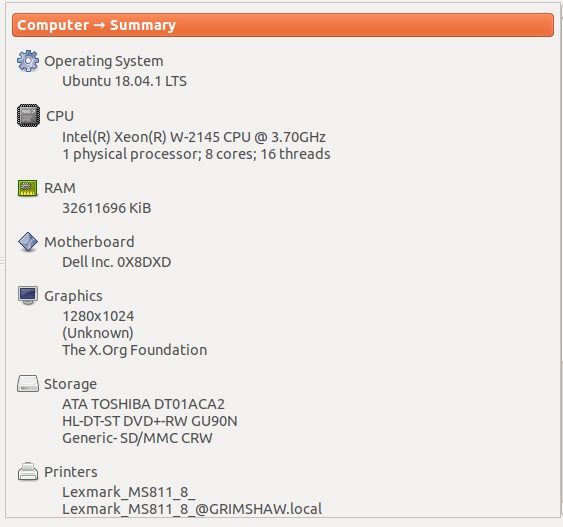
\includegraphics[scale=.5]{hpc}
	\caption{HPC}
	\label{fig:HPC}
\end{figure}

\subsection{Preprocessing}
As mentioned previously in Section~\ref{preproc}, we preprocess the image dataset by using photometric normalisation and \textsc{pca}. 

\subsubsection{Photometric normalisation improves convergence}

Figure~\ref{fig:Compare_Image} shows four examples from the 
\textsc{cifar} dataset. The first two rows illustrate the photometric normalisation effect on the original images. This preprocess technique sharpens the images, and balances their illumination effect by stretching the contrast of ranges. 
The edges of sharpened images are clearer.
Consequently, it improves the convergence of \svm\ dramatically. Meanwhile, normalisation slightly saturates the images.    

\subsubsection{Principal component analysis  speeds up algorithms}

The images preprocessed by \textsc{pca}  (Row~3 in Figure~\ref{fig:Compare_Image}) become blurry compared with the original images. The first $100$ principal component reconstruct $85\%$ of the information in the original image. Although the data size shrinks by more than $30$ times, the structures of the original images still remain.
\begin{figure} 
    \centering
	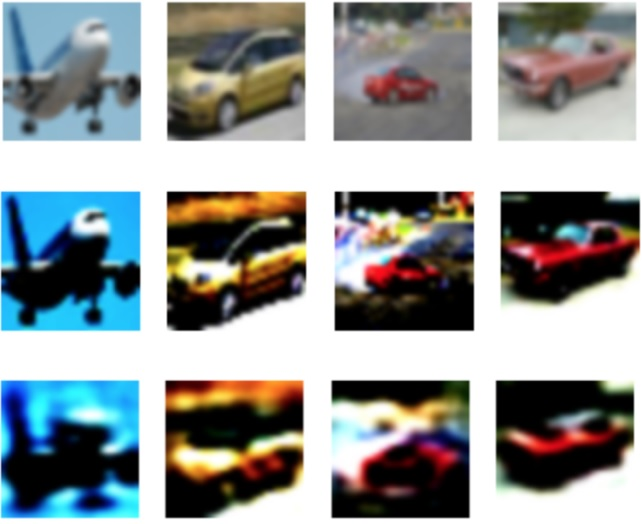
\includegraphics[scale=0.6]{img}
	\caption{Comparison between original images and processed images. The first row shows the original images. The second row shows the images after applying photometric normalisation. The third row shows the \textsc{pca}-processed images.}
	\label{fig:Compare_Image}
\end{figure}

Preprocessing the \textsc{cifar} data with \textsc{pca} speeds up the algorithms by more than 20 times (Table~\ref{tab:Meansd}). While  \textsc{pca} decreases the accuracy of the relabelling algorithm by $3\%$, it increases the accuracy of Expectation Maximisation and Importance Reweighting  by $1.7\%$ and $0.5\%$, respectively. 
\begin{table}
	\caption{Mean, standard deviation and confidence interval of accuracy and average running time for combinations of algorithm and datasets. In the algorithm column, \textsc{em} represents the Expectation Maximisation, \textsc{ir} represents Importance Reweighting and \textsc{r} represents Relabelling. Running time is measured in seconds.}
	\label{tab:Meansd}
\centering
\begin{tabular}{@{}llllll@{}}
\toprule
datset& Algorithm&Mean  & Standard deviation & Confidence interval & Average running time \\ \midrule
&\textsc{em}&0.938 & 0.003              & (0.936,0.939)     & 19.6250\\
\mnist\ &\textsc{ir}&0.94  & 0.003              & (0.939,0.942)     & 73.0786\\
&\textsc{r}&0.942 & 0.003              & (0.941,0.944)     & 65.2899\\
\midrule
&\textsc{em}&0.835 & 0.004              & (0.833,0.837)     & 55.1419\\
\textsc{cifar}&\textsc{ir}&0.844 & 0.005              & (0.841,0.846)     & 283.1319\\
  &\textsc{r}&0.832 & 0.008              & (0.829,0.836)     & 250.8700\\ 
\midrule
\textsc{cifar}&\textsc{em}&0.852 & 0.004              & (0.850,0.853)     & 2.2168\\
 preprocessed&\textsc{ir}& 0.849 & 0.006              & (0.847,0.853)     & 13.8876\\
 by \textsc{pca}  &\textsc{r}& 0.802 & 0.013              & (0.797,0.809)     & 12.2195\\ 
\bottomrule
\end{tabular}
\end{table}



\subsection{Discuss flip rate}

Section~\ref{method2} applies the technique and theorem proposed by \citet{liu2016classification} to estimate the flip rates~$\rhoz$ and $\rhoo$. Our estimations~$\tilde{\rho}_{-1}$ and $\tilde{\rho}_{+1}$ are $0.233$ and $0.35$, respectively. They estimate the true flip rates~$\rhoz=0.2$ and $\rhoo=0.4$ well. 
The estimation~$\tilde{\rho}_{-1}$ is $16.5\%$ greater than the true rate~$\rhoz$, whereas estimation~$\tilde{\rho}_{+1}$ is $12.5\%$ less than  the true rate~$\rhoo$.

There are two possible reasons explaining the errors. 
Firstly, the high dimensionality of the data sets limits the accuracy of estimating probability~$P_{D_\rho}(S|X)$ using density ratio estimation  (Section~\ref{method22}). 
Secondly, the minimum of conditional probabilities of $P_{D_\rho}(S|X)$ is only an estimate of flip rates as described in Section~\ref{method23}.


\subsection{Hyperparameter Tuning}
{\color{red} \\
just states the result hyperparameter from the python file.}
\textsc{em} once
\textsc{ir} twice
\textsc{r} twice


\subsection{Regression estimates running time}
{\color{red} something added}
Figure~\ref{fig:speed} shows that overall, training with \textsc{pca}-processed \textsc{cifar} dataset of dimension $100$ is faster than training with \mnist\ dataset of dimension $784$. 
For either dataset, Expectation Maximisation is the fastest algorithm. Importance Reweighting and Relabelling have similar running time with Relabelling slightly faster.

However, asymptotically, these three algorithms seem to have the same complexity~$\mathcal{O}(n^2p)$. Comparing the same method across different dataset gives the complexity in feature~$p$. For example, when sample size~$n=10,000$, the two rightmost red data points with shapes square and dot in Figure~\ref{fig:speed} illustrate that the running time of the Expectation  algorithm for \mnist\ ($p=784$) and \textsc{pca} preprocessed \textsc{cifar} ($p=100$) are $23$ seconds and $3.3$ seconds. Hence the complexity in sample size~$n$ is 
\begin{math}
    \log(23/3.3)/\log(784/100)=0.94 \approx 1.
\end{math}
Moreover, the slope of the log-log regression in Figure~\ref{fig:speed} are all closed to two, so the complexities of the three algorithms are approximately $\mathcal{O}(n^2p)$ \citep{Roberts:2014:MED:2746455}. 
\begin{figure}
	\centering
    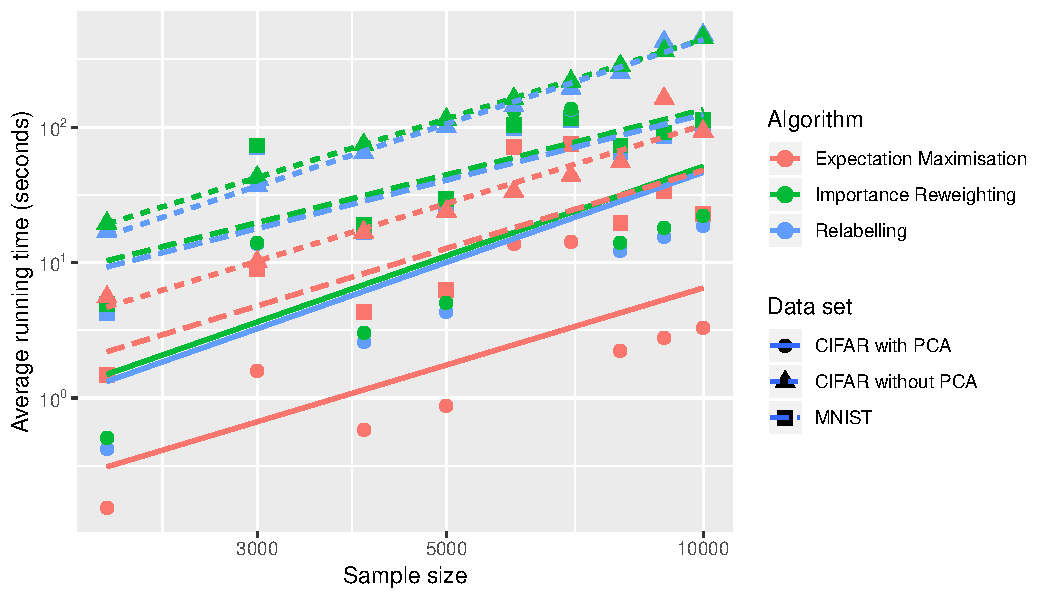
\includegraphics[scale=.8]{speed}%maybe use the large one
	\caption{ Number of samples versus average running time on a log-log scale. The slope of the straight lines on this scale approximates the computational complexity in sample size~$n$. The ratio for a pair of points from the same algorithm and sample size approximates complexity in number of features~$p$.
}
	\label{fig:speed}
\end{figure}
\subsection{Compare algorithms and datasets}

Table~\ref{tab:Meansd} records the descriptive statistics of $16$ Monte Carlo simulations for the three algorithms detailed in Sections~\ref{1st}, \ref{3rd} and~\ref{2nd}.  We test each of the algorithms with datsets \mnist\ and \textsc{cifar}.


\subsubsection{Expectation Maximisation is the fastest}
The rightmost column of Table~\ref{tab:Meansd} illustrates the running time of the three algorithms on the two datsets.
The method of Expectation Maximisation is more than four times faster than the other two methods.

There are two  causes for the difference in speed.
Firstly, the method of Expectation Maximisation only requires to train the base \svm\ model once.
In contrast to Expectation Maximisation, the other two methods all require a pre-training step that predicts the conditional probabilities~$P(S|X)$.
Secondly and most importantly, the loss function~\eqref{eq:dual3} knows the structure of the label noises. Hence, it converges much faster than the other two methods.
In this pre-training step, the method of relabelling and the method of Importance Reweighting have no adequate information about the \textsc{ccn}.
The lack of \textsc{ccn} information slows down the convergence of the algorithms.

\subsubsection{\textsc{cifar} is more difficult to classify}
In terms of accuracy, all algorithms perform significantly better classifying the images in \mnist\ in comparison with classifying images in \textsc{cifar}.
A possible explanation for this might be that \textsc{cifar} is much more complex in nature---it requires $100$ principal components to reconstruct $85\%$ of the image information, where as \mnist\ datset only needs $40$ such principal components.
This observation are also visualised box plot in Figure~\ref{fig:Boxplot}. This figure plots the accuracy of the three algorithms against running time using box plot. For the \mnist\  datset, it seems that the relabelling method are marginally more accurate than the other two algorithms. However, for the  more complex \textsc{cifar} datset, the Importance reweighting seems to be significantly more accurate.
\begin{figure}
	%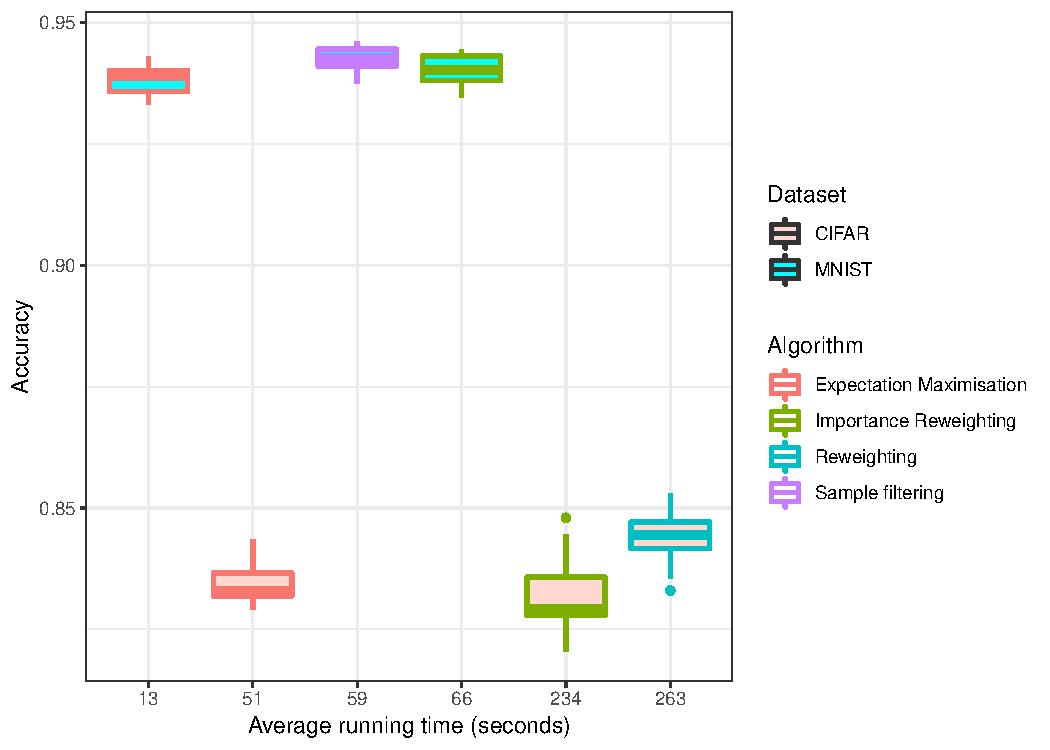
\includegraphics[scale=0.9]{boxplot}
	\centering
    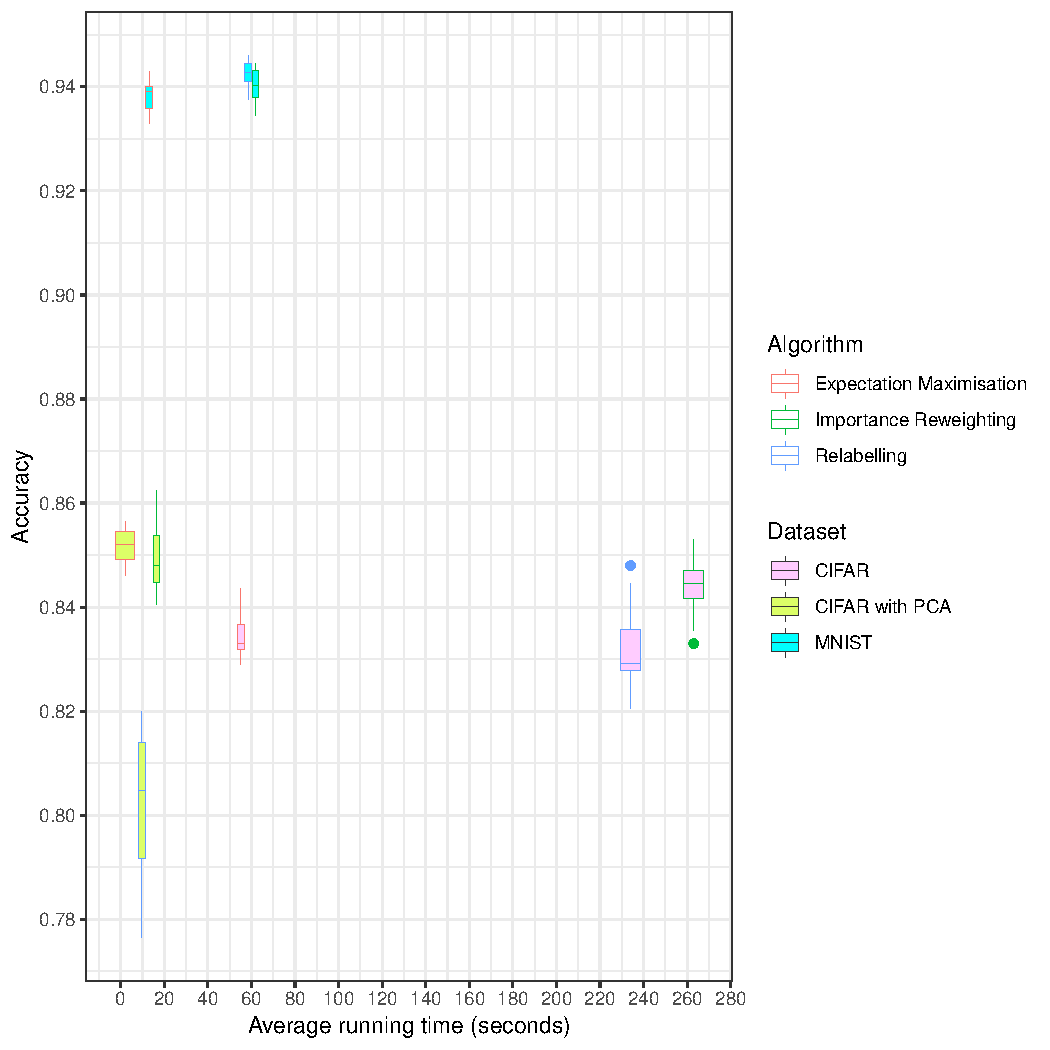
\includegraphics[scale=0.7]{boxplotv}%maybe use the large one
	\caption{Box plots of the accuracy results against running time. Different colours of borders represent different learning algorithms. Different colours filling the boxes represent the two original datasets and \textsc{pca} preprocessed \textsc{cifar}. The vertical edges of boxes represent the $1$st and $3$rd quantiles of accuracy for each setting, and the end of vertical lines represent $1.5$ inter quantile range from these two quantiles. The dots are outliers. 
The right two boxes and the third bottom middle pink box are accuracy classifying original \textsc{cifar} dataset. The bottom left three boxes are accuracy of classifying the \textsc{cifar} dataset with \textsc{pca}. The top left three boxes are accuracy classifying \mnist\ dataset.}
	\label{fig:Boxplot}
\end{figure}

\begin{figure}
	\centering
    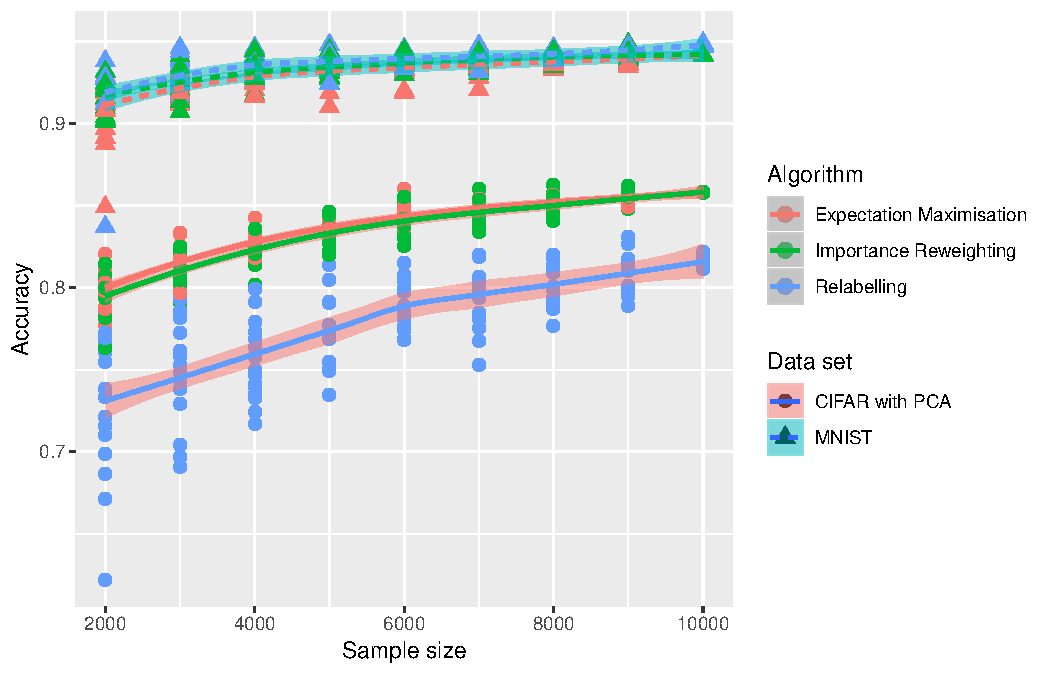
\includegraphics[scale=.8]{accuracy}%maybe use the large one
	\caption{The accuracy of algorithms versus sample size for all three methods on both datasets. The sample size increases from $2,000$ to $10,000$. The coloured regions near the lines indicate a $95\%$ confidence interval. Three colours of the lines represent different algorithms. The three node shapes and the colours filling the confidence intervals correspond to different datasets. 
}
	\label{fig:acc}
\end{figure}

\subsubsection{Relabelling approach is inconsistent and less robust}
When classifying the \textsc{cifar} datset, the wide $95\%$ confidence intervals in accuracy (Table~\ref{tab:Meansd} and Figure~\ref{fig:acc}) suggest that the method of relabelling gives inconsistent classification results against \textsc{ccn}. 
This method only uses $2/3$ of the sample that are believed to be less contaminated. Smaller effective sample size implies greater generalisation errors, and makes this algorithm less consistent. 
Figure~\ref{fig:acc} support this intuition---this method becomes more consistent when the sample size is increased to $n=10,000$.

The inconsistency may also be a consequence of the heuristic nature of the method as described in Section~\ref{2nd}. No asymptotic properties were prove for the process of relabelling. In contrast, Expectation Maximisation method and Importance Reweighting method are mathematically justified. For example, Section~\ref{1st} mathematically derives the choice of the loss function~\eqref{eq:dual3} by Expectation Maximisation.
Similarly, \citet{liu2016classification} give rigorous proofs justifying the properties of the Importance Reweighting formula~\eqref{eq:weighting}. As a result of solid theoretical support, these two methods produce more consistent results.



The inconsistency is not observed in dataset~\mnist. This may partly be explained by the complexity of the datset. For the \mnist\ data ($784$ dimensional), a sample of $8,000$ images is large. However, for the \textsc{cifar} data, the sample size of $8,000$ is on a similar scale with the dimensionality ($3072$).


%\begin{figure}
	%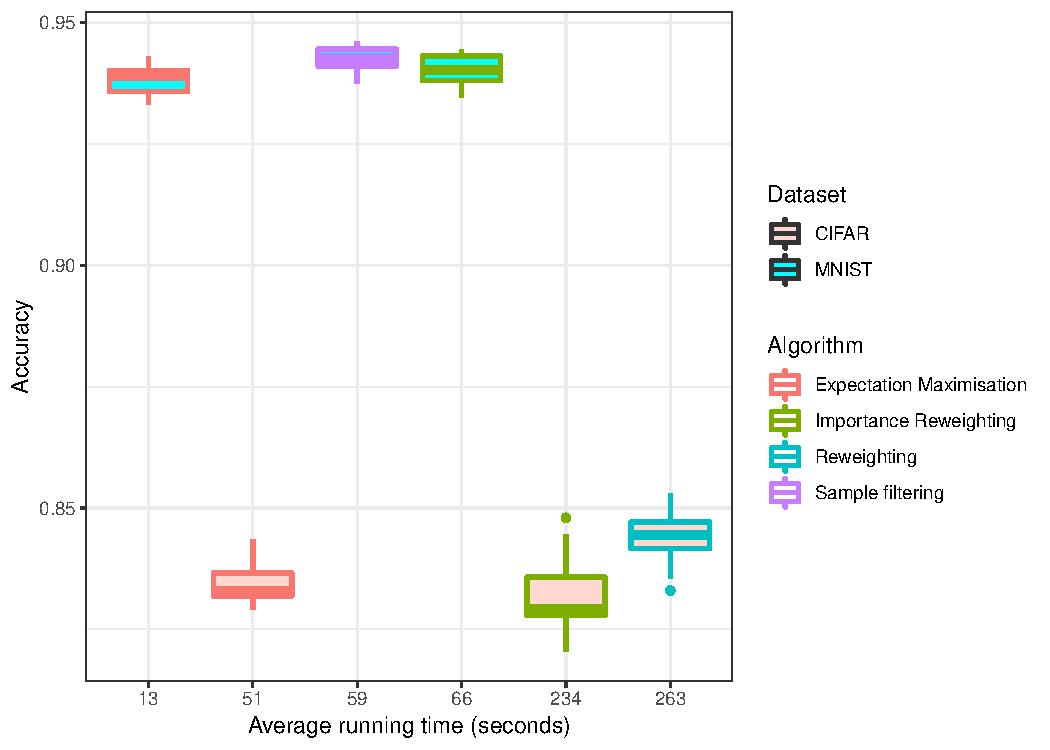
\includegraphics[scale=0.9]{boxplot}
%	\centering
%    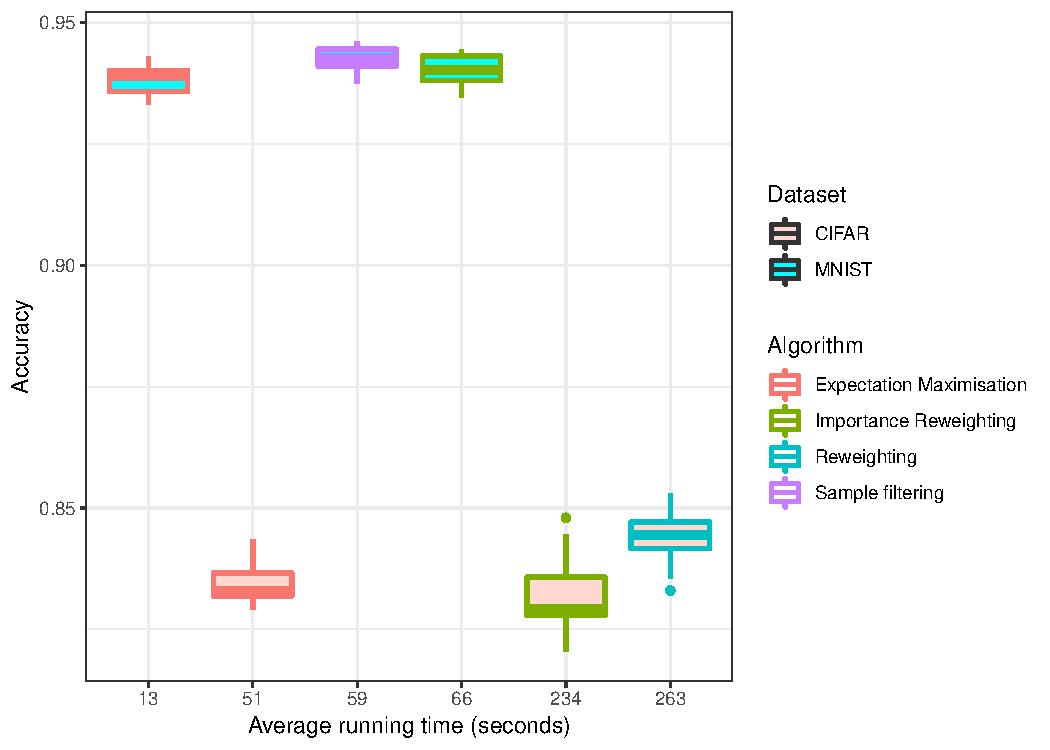
\includegraphics[scale=0.8]{boxplot}%maybe use the large one
%	\caption{Box plots of the accuracy results against running time. {\color{red}Describe various lines and the dots as well as colours here. }
%}
%	\label{fig:Boxplot}
%\end{figure}
\subsubsection{Hypothesis tests justify visualisations}
Kolmogorov-Smirnov test results using the statistic~\eqref{teststatistic} support the visualisations observed from the box plot~\ref{fig:Boxplot}.
\begin{table}%please exchange row 2 3.
\centering
 	\caption{The result of hypothesis test. The result is `reject' indicates we have  statistical evidence at $95\%$ confidence level to conclude one algorithm is more accurate than the other.}
	\begin{tabular}{lllll}
\toprule
Data & $H_0$ & $D$ & P-value & Test result\\
\midrule
 & $A_1= A_2$  &0.3125 & 0.4154 & Fail to reject\\

\mnist & $A_1= A_3$ & 0.625 & 0.0038 & Reject\\

  & $A_2= A_3$ & 0.3125 & 0.4154 & Fail to reject\\
\midrule
   & $A_1= A_2$ & 0.6875 & 0.0010 & Reject\\

 \textsc{cifar}  & $A_1= A_3$ & 0.5 & 0.0366 & Reject\\

  &  $A_2=A_3$  & 0.6875 & 0.0010 & Reject\\
 \midrule
  \textsc{cifar} & $A_1= A_2$ & 0.375 & 0.2106 & Fail to reject\\

  preprocessed & $A_1= A_3$ & 1 & 0 & Reject\\

  by \textsc{pca} &  $A_2=A_3$  & 1 & 0 & Reject\\
\bottomrule
\end{tabular}

	\label{tab:HypothesisTest}
\end{table}
As illustrated in  Table~\ref{tab:HypothesisTest}, the test statistic ($D=0.625>0.433$) suggests that the relabelling method ($A_3$) more accurately classifies the \mnist\ datset with label noise, comparing with the Expectation Maximisation method ($A_1$).
However, the hypothesis test are not able to conclude whether Importance Reweighting ($A_2$) outperforms or is outperformed by the other two algorithm with these $16$ simulations of accuracy results, for \mnist\ datset.

In terms of \textsc{cifar} datset, there are strong statistical evidences suggesting Importance Reweighting method classifies the images in the noisy \textsc{cifar} datset more accurately than the expectation maximisation method. Similarly, and we are also $95\%$ confident to accept the hypothesis that the Expectation Maximisation method is more accurate than the importance relabelling method.

Density plot~\ref{fig:Density} of the accuracy results visualise these results concluded by Kolmogorov-Smirnov hypothesis tests.
\begin{figure}
    \centering
	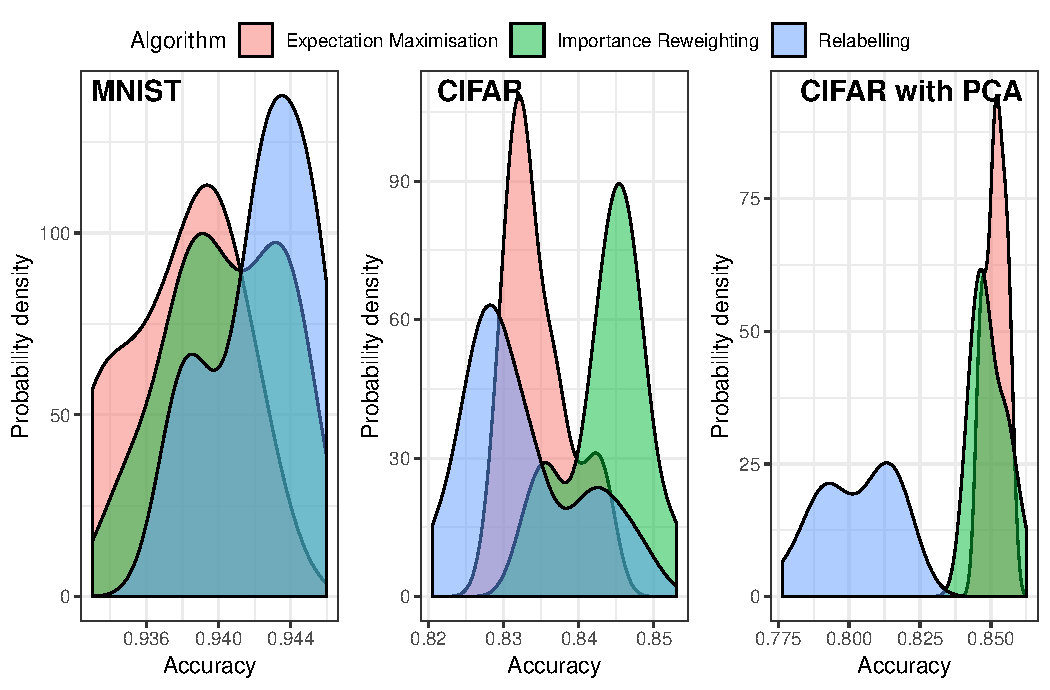
\includegraphics[scale=0.8]{histo}
	\caption{Density function from kernel smoothing. Left is mid is right is pink is green is blue is.}
	\label{fig:Density}
	%Then we estimate the density function using kernel smoothing and plot figure \ref{fig:Density function from kernel smoothing}.
\end{figure}




\subsection{Discussion and personal reflection}
%Please write these in full good English sentences.

%\textsc{em} is fast, require good estimate of $\rho$. Need mathematical derivation of objective function. Derivation depends on base method and error distribution, needs mathematical skills. Low accuracy due to it only minimise a upper bound of the true loss function. From optimisation point of view, this is equivalent to a local minimum \citep{NIPS1999_1672}.

%Relabelling no need to know $\rho$. However, in consistent result. Only useful with large data.
%Select a region where $P(S=g(x))$ is high where $g(x)$ is the decision function~\eqref{eq:decision}.

%Reweighting is the best overall, more accurate and consistent.

The three methods introduced in Sections~\ref{1st}, \ref{3rd} and \ref{2nd}  all perform well against \textsc{ccn} when testing with the datsets~\mnist\ ($A\approx 94\%$) and~\textsc{cifar} ($A\approx 85\%$). However, the relabelling method proposed in Section~\ref{2nd} does not classify the \textsc{cifar} datset well ($A\approx 80\%$) when preprocessed with \textsc{pca}. Nevertheless, preprocessing with \textsc{pca} improves the speed of each algorithm by approximately 20 times. Surprisingly, \textsc{pca} also marginally improves the accuracy of the Expectation Maximisation method ($3\%$) and the Importance Reweighting method ($1\%$), perhaps by decreasing the generalisation error.


Our work finds that Expectation Maximisation is significantly faster than the other two algorithms. This might be a consequence of carefully designed loss function. In addition, the requirement of a pre-training model to predict the conditional probabilities dramatically increases the computational complexity of Important Reweighting and relabelling algorithms. Although Expectation Maximisation is computational efficient, it requires mathematical derivations of several moments of the noise distribution and involved modifications of the base algorithm. This procedure can be error-prone and might be challenging for data scientists with minimal mathematical background. For \svm , this modification ends up being a straightforward Hadamard matrix multiplication correction on the Kernel matrix, as detailed in Section~\ref{sec:mod}. Further, Expectation Maximisation is theoretically less sound in comparison to Importance Reweighting rigorous proposed by \citet{liu2016classification}. The former method only minimises an upper bound of the true loss function \citep{NIPS1999_1672}. Thus, Expectation Maximisation only assures us the selected parameters are a local optimum.

In contrast, the Importance Reweighting method provides an easy-to-follow structured approach against binary classification problem with \textsc{ccn}. As a result, this approach is likely to be more popular in the commercial world. Also, \citet{liu2016classification} proved theorems which guarantee the performance of this approach under reasonable assumptions. As regards performance, the Importance Reweighting method outperforms Expectation Maximisation when we only have a moderated number of samples comparing with dimensionality (i.e. \textsc{cifar} without \textsc{pca}). This observation may suggest that Importance Reweighting method has a better convergence rate. 

The heuristically proposed relabelling algorithm does not requires flip rates as an input. But, it gives inconsistent classification results, unless the sample size is prohibitively larger than the number of features in the input datset.  Hence, we only recommend this `quick and dirty' approach for large datsets with simple structures. 

%\subsection{Backup Statements}









%{\color{red} please plot the cifar with and without PCA, put them into one graph and compare. codes are already available. just run them and save and insert.}

%We use the methods,\ref{1st}, \ref{2nd} and \ref{3rd}, to conduct experiments on two datasets, fashion-mnist and \textsc{cifar}.
%Both datasets are re-organized to have two classes 0 and 1.
%For clearer notation, we refer to class 0 as -1 and class 1 as +1.
%Both datasets have flip rates $\rhoz=0.2$ and $\rhoo=0.4$.
%The fashion-mnist has dimension $d=784$, while \textsc{cifar} has $d=3072$.
%{\color{red} original image}
%As mentioned in section \ref{preproc}, we need to run \textsc{pca} on \textsc{cifar} to reduce the dimensionality.



\section{Conclusion}
This main goal of this report is to implement and compare the three algorithms classifying images with \textsc{ccn} as described in Sections~\ref{1st}, \ref{3rd} and~\ref{2nd}. 
Multiple nonparametric regression analysis and hypothesis tests revealed that the relabelling algorithm is less robust to label noise than Expectation Maximisation and Importance Reweighting methods, especially for complex datsets. Meanwhile, Importance Reweighting method is more sound theoretically \citep{liu2016classification} and is easier to implement than Expectation Maximisation. 
Despite of its longer training time, we numerically justified that its computational complexity is the same as Expectation Maximisation.
In general, therefore, it seems that the Importance Reweighing method is the best algorithm among these three. 
Our results provided extra numerical complements to the theoretical work done by \citet{liu2016classification}. 

The major limitation of this study is the number of datset tested. Our finding are only based on the performance classifying the datsets~\mnist\ and~\textsc{cifar}. A natural progression of this work is to analyse these three methods on more datsets with \textsc{ccn} and draw a reasonable hypothesis on the asymptotic behaviours of the algorithms. Ideally, these asymptotic properties need to be rigorous proved. Also, our hyperparameters are tuned such that the training accuracy matches the given flip rates (i.e. $0.7$). Dr. Liu invited us to explore the possibility to give a theoretical justification of this tuning method under his supervision.
\label{headings}

\bibliographystyle{unsrtnat}
\bibliography{reference}

\end{document}
